% Presentación de PULSO, versión 3: exposición de 30 minutos.
% 25 diapositivas principales (unos 28 minutos) y diapositivas de respaldo para preguntas.
% El texto de cada diapositiva está en el guion (docs/latex/guion_v3).
% Compilar desde docs/latex/presentacion_v3:
%   latexmk -lualatex presentacion_v3.tex
\documentclass[aspectratio=169,11pt]{beamer}
\usetheme[progressbar=frametitle,numbering=fraction,block=fill,sectionpage=progressbar]{metropolis}
\usepackage{appendixnumberbeamer}
\usepackage{fontspec}
\usepackage[spanish,es-noshorthands,es-nodecimaldot]{babel}
\usepackage{amsmath,amssymb}
\usepackage{booktabs}
\usepackage{tikz}
\usetikzlibrary{arrows.meta,positioning,calc,decorations.pathreplacing}
\usepackage[most]{tcolorbox}
\setmonofont{DejaVu Sans Mono}[Scale=0.78]
\graphicspath{{../figuras/}{../../../figures/}}

\definecolor{azul}{HTML}{2563A8}
\definecolor{rojo}{HTML}{C2362B}
\definecolor{verde}{HTML}{2F7D5B}
\definecolor{ambar}{HTML}{C98F00}
\definecolor{morado}{HTML}{7B4FA0}
\definecolor{gris}{HTML}{5F6B77}
\setbeamercolor{frametitle}{bg=azul}
\setbeamercolor{progress bar}{fg=rojo}
\setbeamercolor{alerted text}{fg=rojo}
\setbeamercolor{block title}{bg=azul!15,fg=black}
\setbeamercolor{block body}{bg=azul!5}
\setbeamercolor{block title alerted}{bg=rojo!15,fg=black}
\setbeamercolor{block body alerted}{bg=rojo!5}
\setbeamercolor{block title example}{bg=verde!15,fg=black}
\setbeamercolor{block body example}{bg=verde!5}

% Mensaje clave al pie de cada diapositiva: una sola idea para recordar.
\newcommand{\clave}[1]{\vfill
  \begin{tcolorbox}[colback=azul!9,colframe=azul!9,boxrule=0pt,arc=2pt,
    left=6pt,right=6pt,top=3pt,bottom=3pt,fontupper=\small\bfseries\color{azul!70!black}]
  #1\end{tcolorbox}}

\tikzset{
  caja/.style={draw=#1,fill=#1!8,rounded corners=3pt,align=center,
    minimum height=1.0cm,font=\small},
  f/.style={-{Stealth[length=2.5mm]},thick,gris}}

\title{PULSO}
\subtitle{Pagos, Umbrales, Liquidez y Sincronización Operativa\\[2pt]
\footnotesize Redes complejas, sincronización y riesgo en sistemas de pagos digitales}
\author{Juan Diego Martínez Ayala \\ \small Dirección: Jhon Hernán Díaz Forero}
\institute{\small Semillero de Modelamiento de Sistemas Complejos y Física Computacional}
\date{Noviembre de 2026}

\begin{document}
\maketitle

% ===================================================================
\section{El problema}

\begin{frame}{Los pagos forman una red y los problemas viajan por ella}
\begin{columns}[c]
\column{0.5\textwidth}
\begin{itemize}
\item Cada persona y cada empresa paga con lo que recibe de otras.
\item Si alguien deja de pagar, sus receptores reciben menos.
\item Con pagos inmediatos (Bre-B), el problema también se transmite más rápido.
\end{itemize}
\column{0.46\textwidth}
\centering
\begin{tikzpicture}[n/.style={circle,draw=azul,fill=azul!10,minimum size=8mm,font=\small},
  e/.style={-{Stealth[length=2.2mm]},thick}]
\node[n,fill=rojo!45] (a) at (0,0) {A};
\node[n] (b) at (2,0.9) {B};
\node[n] (c) at (2,-0.9) {C};
\node[n] (d) at (4,0) {D};
\draw[e] (a)--(b); \draw[e] (a)--(c); \draw[e] (b)--(d); \draw[e] (c)--(d);
\node[font=\footnotesize,align=center] at (2,-1.9) {A deja de pagar: B y C reciben menos\\y D se afecta sin relacionarse con A};
\end{tikzpicture}
\end{columns}
\clave{Un problema de liquidez no se queda donde empieza.}
\end{frame}

\begin{frame}{No solo importa cuánto se recibe, también cuándo}
\centering
\begin{tikzpicture}[x=0.28cm,y=1cm]
\foreach \y/\lab/\col/\s in {1.6/{En fase}/verde/28, 0/{Desfasado}/rojo/38}{
  \node[anchor=east,font=\small\bfseries,text=\col] at (-0.8,\y) {\lab};
  \draw[gris,thick] (0,\y)--(40,\y);
  \foreach \d in {0,10,20,30,40} \draw[gris] (\d,\y-0.08)--(\d,\y+0.08);
  \draw[very thick,azul] (35,\y-0.22)--(35,\y+0.22);
  \node[above,font=\scriptsize,text=azul] at (35,\y+0.22) {cuota};
  \fill[\col] (\s,\y) circle (4.5pt);
  \node[below,font=\scriptsize,text=\col] at (\s,\y-0.15) {salario};
}
\draw[rojo,line width=3pt,opacity=0.5] (35,0)--(38,0);
\node[font=\scriptsize\bfseries,text=rojo] at (24,-0.45) {3 días sin liquidez $\rightarrow$};
\foreach \d/\t in {0/{día 0},10/{10},20/{20},30/{30},40/{40}}
  \node[font=\scriptsize,gris] at (\d,-1.0) {\t};
\end{tikzpicture}

\vspace{0.2cm}
\begin{itemize}
\item Mismo salario, misma cuota. Solo cambia la fecha de llegada del ingreso.
\item Al ingreso que llega tarde respecto a las obligaciones lo llamamos
\alert{desfase} o \alert{desincronización}.
\end{itemize}
\clave{El ingreso desfasado genera estrés aunque el monto no cambie.}
\end{frame}

\begin{frame}{Pregunta de investigación}
\begin{block}{Pregunta}
¿La \textbf{sincronización} de los ciclos de pago, estimada solo con las transacciones de
un banco, ayuda a predecir el \textbf{impago} mejor que
\begin{enumerate}
\item el \textbf{score clásico} (ingreso, deuda, mora), y
\item la \textbf{red estática} (quién le paga a quién y cuánto)?
\end{enumerate}
\end{block}
\begin{exampleblock}{Hipótesis falsable}
Si el desfase genera déficit, la sincronización mejora la predicción. Si no lo genera
(\textbf{control nulo}), no la mejora.
\end{exampleblock}
\clave{Comparamos contra la red estática porque eso ya existe en la literatura.}
\end{frame}

\begin{frame}{Seis tareas, un solo modelo}
\centering
\begin{tikzpicture}[node distance=0.2cm,every node/.append style={font=\footnotesize}]
\node[caja=azul,minimum width=2.05cm] (t1) {\textbf{1}\\Red y\\déficit};
\node[caja=azul,minimum width=2.05cm,right=of t1] (t2) {\textbf{2}\\Redistri-\\bución};
\node[caja=azul,minimum width=2.05cm,right=of t2] (t3) {\textbf{3}\\Sincroni-\\zación};
\node[caja=azul,minimum width=2.05cm,right=of t3] (t4) {\textbf{4}\\Impagos y\\cascadas};
\node[caja=azul,minimum width=2.05cm,right=of t4] (t5) {\textbf{5}\\Predicción\\con ML};
\node[caja=rojo,minimum width=2.05cm,right=of t5] (t6) {\textbf{6}\\Riesgo de\\crédito};
\foreach \a/\b in {t1/t2,t2/t3,t3/t4,t4/t5,t5/t6} \draw[f] (\a)--(\b);
\draw[decorate,decoration={brace,mirror,amplitude=6pt},thick,gris]
  ($(t1.south west)+(0,-0.15)$)--($(t5.south east)+(0,-0.15)$)
  node[midway,below=8pt,font=\small,text=gris] {propuesta del semillero: construir el modelo};
\node[below=0.55cm of t6,font=\small,text=rojo,align=center] {aplicación\\a un banco};
\end{tikzpicture}

\vspace{0.4cm}
Cada tarea agrega un término al modelo. Con ese término apagado, el modelo vuelve
\textbf{exactamente} a la tarea anterior.
\clave{Cada pieza se valida antes de agregar la siguiente.}
\end{frame}

% ===================================================================
\section{El modelo}

\begin{frame}{La ecuación del déficit}
\[
\frac{dx_i}{dt} = \underbrace{\color{verde}-\alpha x_i}_{\text{corrección}}
+ \underbrace{\color{rojo}\beta\sum_j W_{ij}x_j}_{\text{contagio}}
\underbrace{\color{azul}- D_0(Lx)_i}_{\text{redistribución}}
+ \underbrace{\color{morado}\gamma\,k_i(1-r_i)}_{\text{desfase}}
+ \underbrace{\eta_i(t)}_{\text{choques}}
\]
\vspace{0.1cm}
\begin{itemize}
\item $x_i$: \textbf{déficit} de la entidad $i$ (cuánta liquidez le falta).
\item $W_{ij}$: cuánto le paga $j$ a $i$ en cada ciclo.
\item Si $x_i$ supera su \textbf{colchón} $x_i^{(c)}$, la entidad deja de pagar:
\textbf{impago}.
\end{itemize}
\clave{Cinco efectos en una ecuación: se corrige, se contagia, se reparte, se desfasa y
recibe choques.}
\end{frame}

\begin{frame}{La ecuación del ritmo de pagos}
\[
\frac{d\theta_i}{dt} = \omega_i + \frac{K}{\langle k\rangle}\sum_j W_{ij}\sin(\theta_j-\theta_i)
\qquad
r_i = \frac{1}{k_i}\sum_j W_{ij}\cos(\theta_j-\theta_i)
\]
\begin{columns}[c]
\column{0.55\textwidth}
\begin{itemize}
\item $\theta_i$: en qué punto de su ciclo de pagos está $i$ (como la manecilla de un
reloj).
\item Cada entidad ajusta su ritmo al de quienes le pagan: modelo de
\textbf{Kuramoto}.
\item $r_i$: \textbf{coherencia}. $1$ = el ingreso llega a tiempo; $-1$ = llega en
contrafase.
\end{itemize}
\column{0.4\textwidth}
\centering
\begin{tikzpicture}
\draw[gris,thick] (0,0) circle (1.1);
\foreach \a/\c in {80/verde,95/verde,105/verde,250/rojo}{
  \fill[\c] (\a:1.1) circle (3.5pt);}
\draw[-{Stealth},thick,verde] (0,0)--(93:0.85);
\node[font=\scriptsize,text=verde] at (93:1.55) {pagadores en fase};
\node[font=\scriptsize,text=rojo] at (250:1.55) {desfasado};
\end{tikzpicture}
\end{columns}
\clave{El término $\gamma k_i(1-r_i)$ convierte el desfase en déficit: une el ritmo con
la liquidez.}
\end{frame}

% ===================================================================
\section{Lo que muestra el modelo}

\begin{frame}{La red amortigua los choques solo si $R<1$}
\centering
\vspace{0.15cm}
$R=\dfrac{\beta\,\rho(W)}{\alpha}=\dfrac{\text{contagio}}{\text{corrección}}$
\qquad {\small como el número reproductivo de una epidemia}

\vspace{0.15cm}
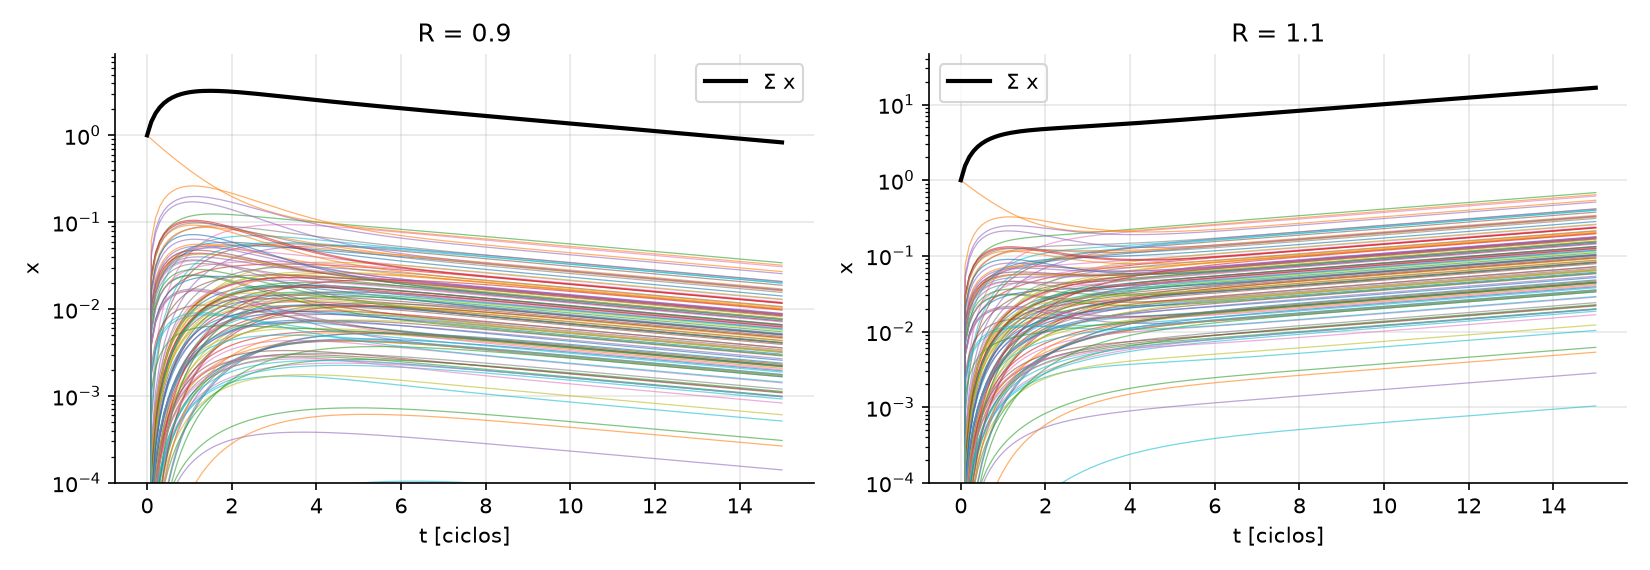
\includegraphics[width=0.78\textwidth]{fase1_trayectorias.png}

{\small Déficit de cada entidad tras un choque (línea negra: total). Verificado contra la
solución exacta, error $<10^{-6}$.}
\clave{Con $R=0.9$ el déficit total se apaga; con $R=1.1$ crece sin límite.}
\end{frame}

\begin{frame}{Los ciclos de pago se sincronizan como predice la teoría}
\begin{columns}[c]
\column{0.4\textwidth}
\small
\begin{itemize}
\item Sincronía global $r$: 0 = cada uno a su ritmo; 1 = todos a la vez.
\item Crece con el acoplamiento $K$.
\item Red completa: teoría $r=\sqrt{1-2\Delta/K}$.
\item Con $K=2$: \textbf{0.7071} teórico, \textbf{0.7076} simulado.
\end{itemize}
\column{0.58\textwidth}
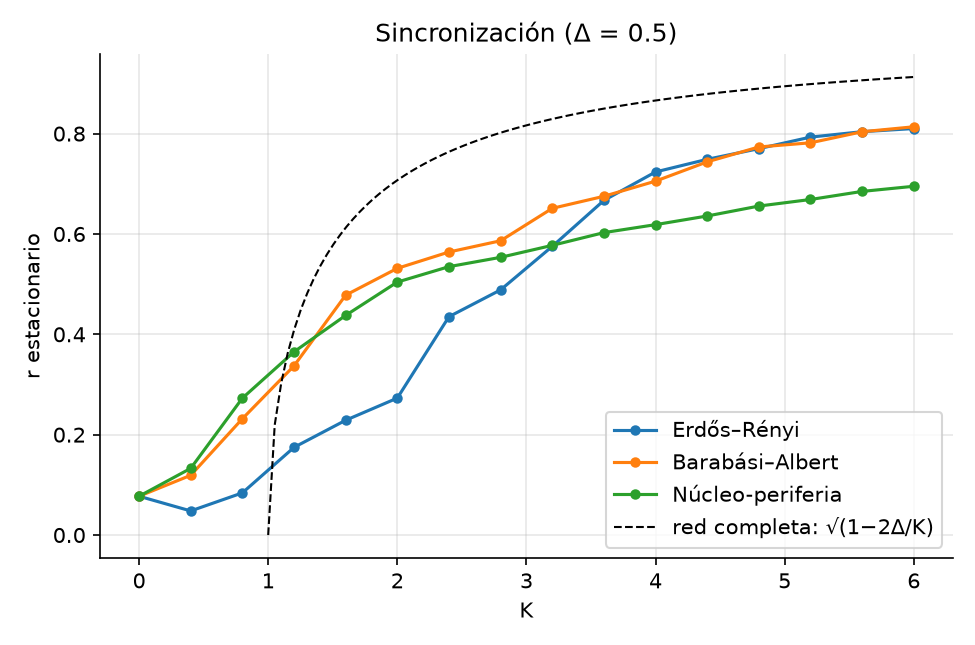
\includegraphics[width=\textwidth]{fase3_r_vs_K.png}
\end{columns}
\clave{El código reproduce un resultado exacto de la física de la sincronización.}
\end{frame}

\begin{frame}{Las cascadas son máximas con conectividad intermedia}
\begin{columns}[c]
\column{0.38\textwidth}
\small
\begin{itemize}
\item Pocas conexiones: el choque no tiene por dónde pasar.
\item Muchas: cada entidad reparte su riesgo y absorbe la pérdida.
\item En medio: \alert{ventana de contagio}.
\end{itemize}
\column{0.6\textwidth}
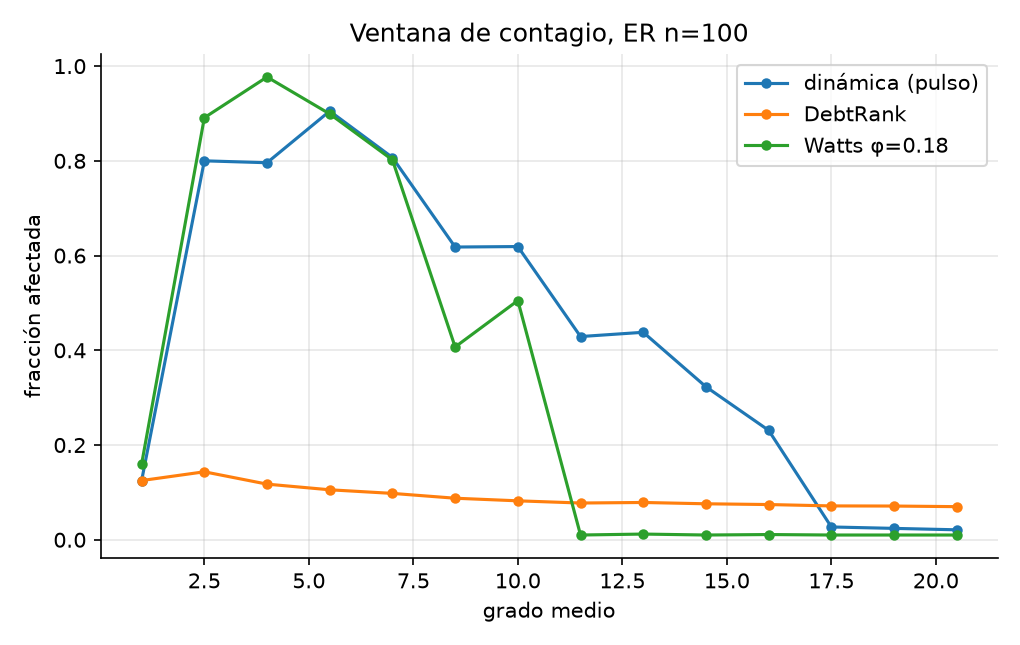
\includegraphics[width=\textwidth]{fase4_ventana_contagio.png}
\end{columns}
\clave{Más conexiones no siempre significa más riesgo.}
\end{frame}

\begin{frame}{El aprendizaje automático predice el colapso en milisegundos}
\begin{columns}[c]
\column{0.45\textwidth}
\begin{itemize}
\item 20\,000 simulaciones sobre 300 redes.
\item XGBoost: \textbf{AUC 0.98} para predecir el colapso global.
\item Simular: 0.08 s. Predecir: 0.2 ms.
\item Validación con redes que el modelo no vio.
\end{itemize}
\column{0.53\textwidth}
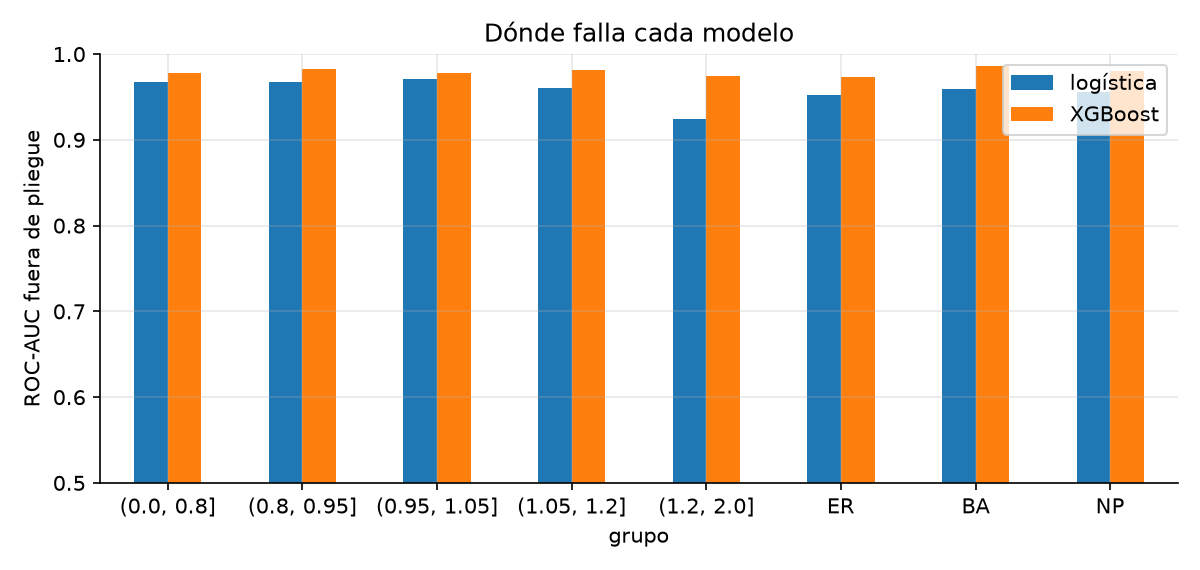
\includegraphics[width=\textwidth]{fase6_comparacion_modelos.png}
\end{columns}
\clave{El modelo físico genera los datos; el aprendizaje automático los resume.}
\end{frame}

% ===================================================================
\section{Aplicación al riesgo de crédito}

\begin{frame}{Una cartera bancaria en tres capas}
\begin{columns}[c]
\column{0.42\textwidth}
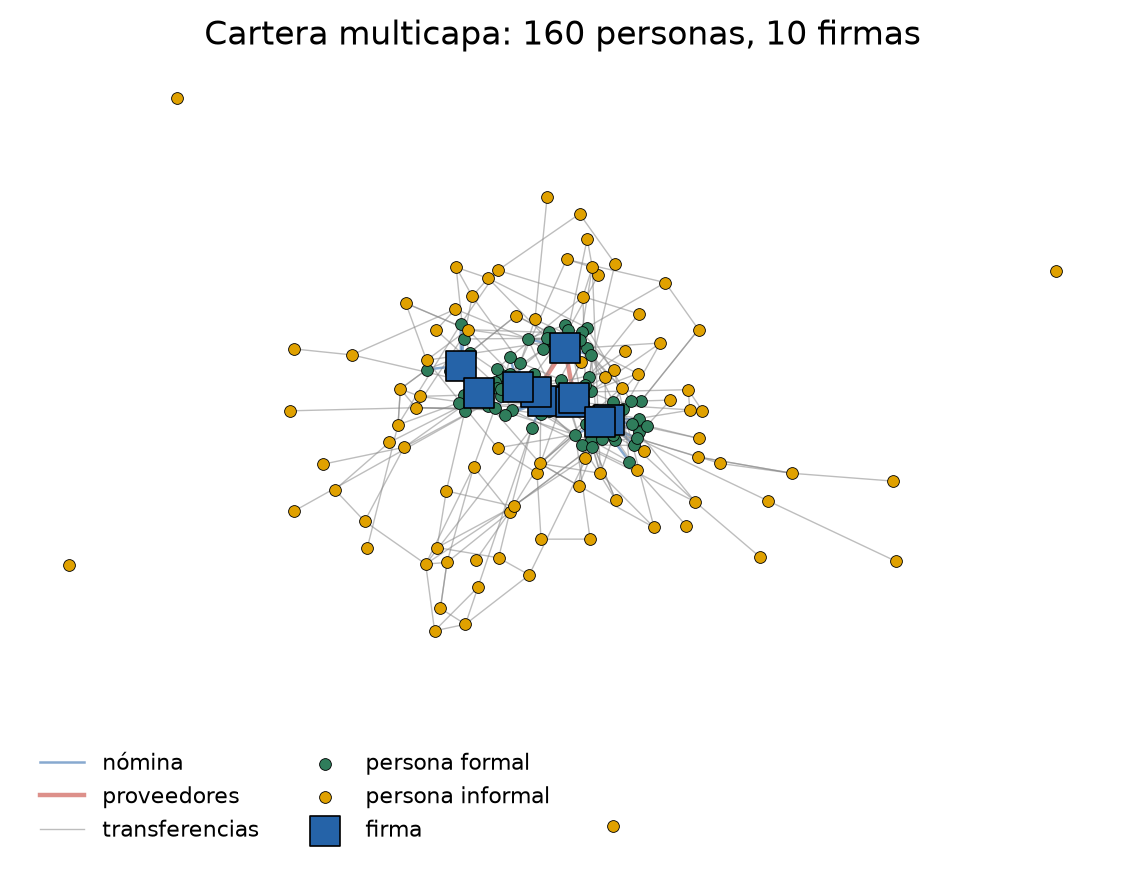
\includegraphics[width=\textwidth]{tarea6_red_multicapa.png}
{\scriptsize Ejemplo reducido para ver las capas.}
\column{0.56\textwidth}
\footnotesize
\begin{tabular}{lll}
\toprule
Capa & De $\to$ a & Ritmo \\
\midrule
\textcolor{azul}{Nómina} & empresa $\to$ persona & 15 o 30 días \\
\textcolor{rojo}{Proveedores} & empresa $\to$ empresa & facturas \\
Transferencias & persona $\to$ persona & irregular \\
\bottomrule
\end{tabular}
\vspace{0.3cm}

2000 personas, 100 empresas, 55~\% de informalidad. Datos \textbf{sintéticos} con un
mecanismo conocido.
\end{columns}
\clave{Se simula una cartera para comprobar que el método encuentra lo que sabemos que
está.}
\end{frame}

\begin{frame}{El banco solo ve transacciones; el ritmo se estima desde ellas}
\begin{columns}[c]
\column{0.42\textwidth}
\small
\begin{enumerate}
\item El modelo genera pagos: fecha, pagador, receptor, monto.
\item Con esos pagos se estima la fase de cada cliente.
\item Con las fases se estima su coherencia $\hat r_i$.
\end{enumerate}
\vspace{0.2cm}
Observar 6 meses; predecir el impago de los 12 siguientes.
\column{0.56\textwidth}
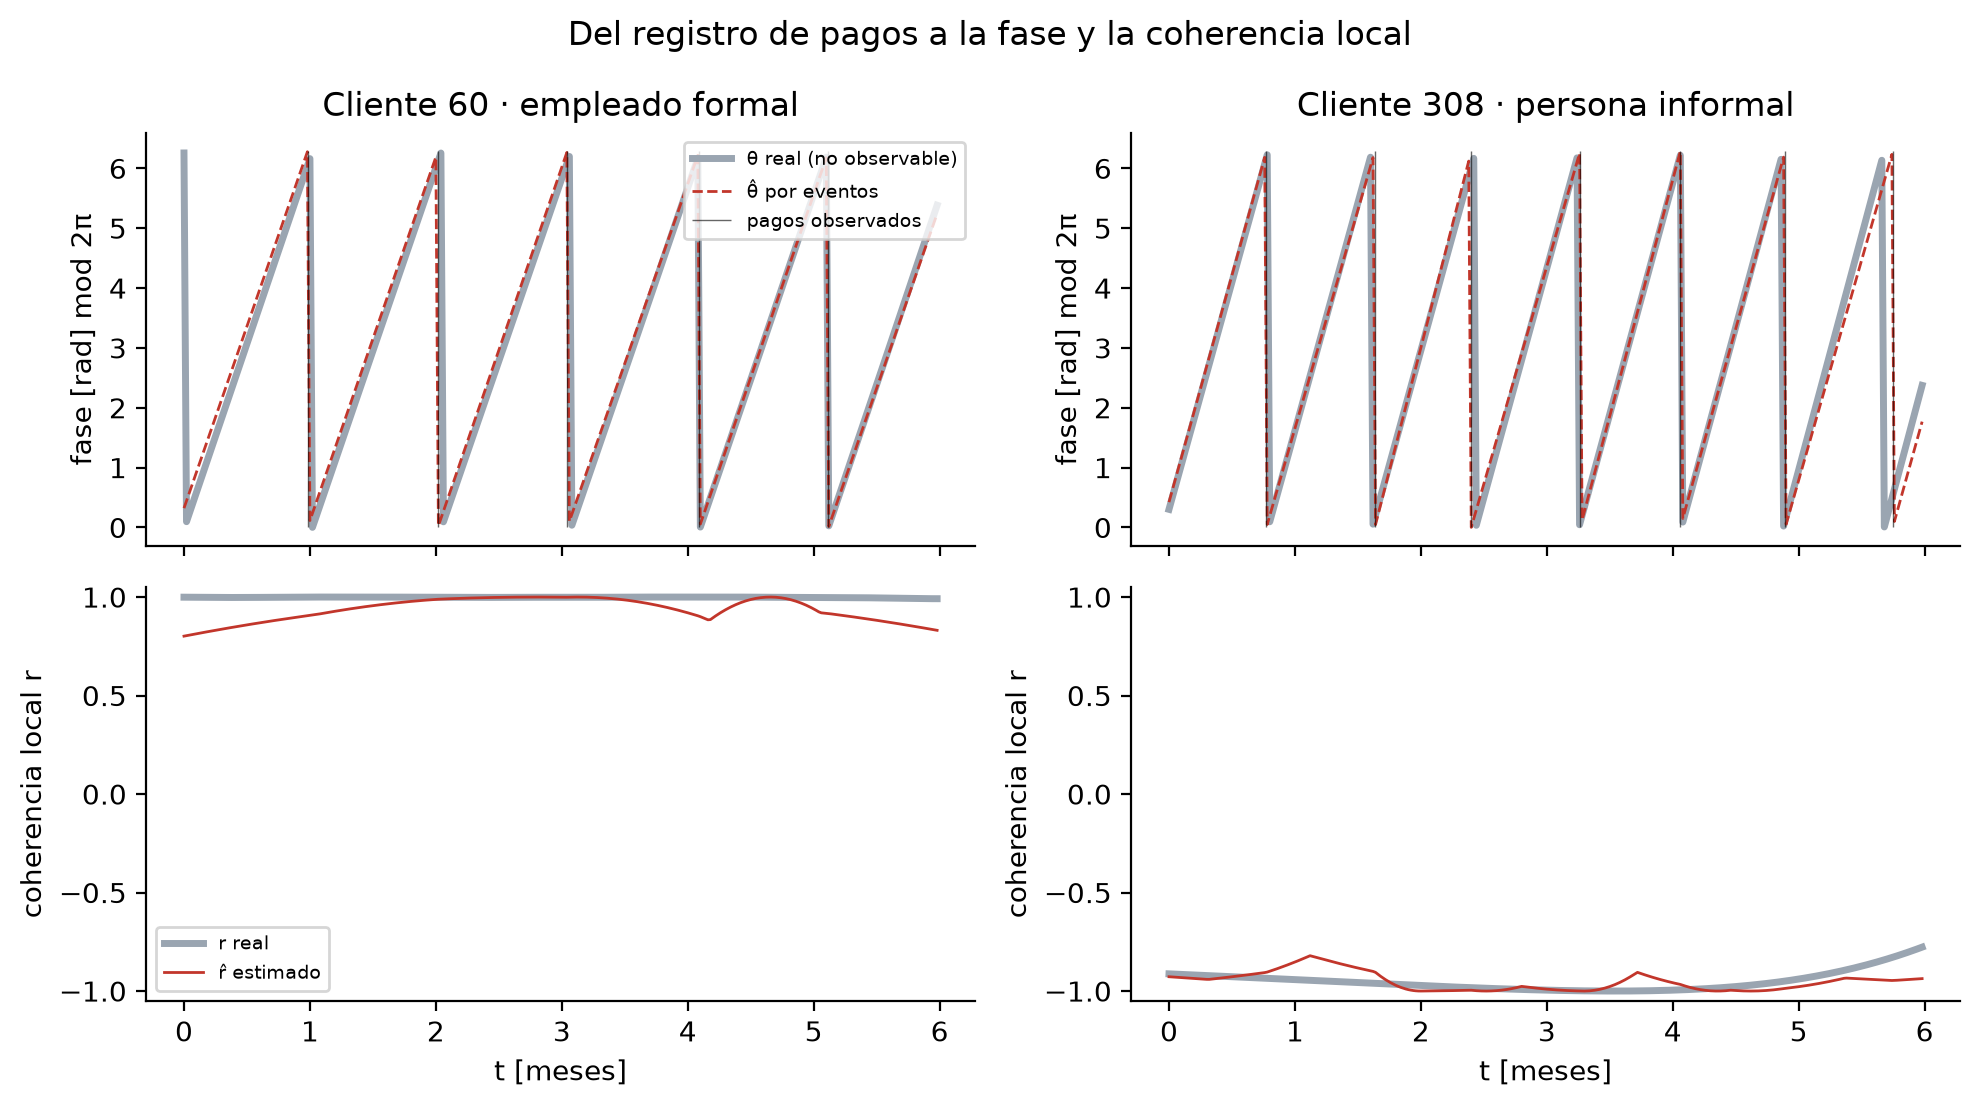
\includegraphics[width=\textwidth]{tarea6_fase_eventos.png}
\end{columns}
\clave{La coherencia estimada coincide con la real (correlación $>0.8$).}
\end{frame}

\begin{frame}{Tres niveles de información}
\centering
\begin{tikzpicture}[node distance=0.2cm]
\node[caja=gris,minimum width=12.5cm,align=left,text width=12cm] (n1)
  {\textbf{1 · Clásico}: ingreso, endeudamiento, edad, antigüedad, moras, formalidad};
\node[caja=azul,minimum width=12.5cm,align=left,text width=12cm,below=of n1] (n2)
  {\textbf{2 · + Red estática}: de quién recibe, cuánto, qué tan concentrado, salud del
  empleador};
\node[caja=rojo,minimum width=12.5cm,align=left,text width=12cm,below=of n2] (n3)
  {\textbf{3 · + Red dinámica}: coherencia $\hat r$, desfase, ritmo, regularidad, pagadores
  que dejaron de pagar};
\end{tikzpicture}

\vspace{0.3cm}
Cada nivel contiene al anterior. Mismo modelo, mismos clientes, misma validación.
\clave{El nivel 3 es el aporte del proyecto.}
\end{frame}

\begin{frame}{El experimento compara dos mundos idénticos}
\centering
\begin{tikzpicture}
\node[font=\small,align=center] (s) at (0,0)
  {mismos clientes · misma red · mismos números aleatorios};
\node[caja=rojo,minimum width=5.6cm,minimum height=2.0cm,text width=5.2cm] (r) at (-3.4,-2.0)
  {\textbf{Mundo con red}\\[3pt]el desfase y el contagio\\generan déficit};
\node[caja=gris,minimum width=5.6cm,minimum height=2.0cm,text width=5.2cm] (n) at (3.4,-2.0)
  {\textbf{Mundo nulo (control)}\\[3pt]los pagos existen, pero\\no generan déficit};
\draw[f] (s.south)--(r.north); \draw[f] (s.south)--(n.north);
\node[below=0.2cm of r,font=\small,text=rojo] {la dinámica \emph{debería} ayudar};
\node[below=0.2cm of n,font=\small,text=gris] {la dinámica \emph{no debería} ayudar};
\end{tikzpicture}

\vspace{0.3cm}
\small 20 carteras por mundo, unos 40\,000 clientes. Validación cruzada por cartera.
\clave{Si la dinámica mejorara también en el mundo nulo, el método estaría engañando.}
\end{frame}

% ===================================================================
\section{Resultados}

\begin{frame}{Cada nivel de información mejora la predicción}
\centering
\begin{tikzpicture}[node distance=1.5cm]
\node[caja=gris,minimum width=3.4cm,minimum height=1.6cm] (a)
  {\textbf{1 · Clásico}\\[2pt]{\Large 0.769}};
\node[caja=azul,minimum width=3.4cm,minimum height=1.6cm,right=of a] (b)
  {\textbf{2 · + Estática}\\[2pt]{\Large 0.784}};
\node[caja=rojo,minimum width=3.4cm,minimum height=1.6cm,right=of b] (c)
  {\textbf{3 · + Dinámica}\\[2pt]{\Large\bfseries 0.795}};
\draw[f] (a)--node[above,font=\scriptsize]{+0.015}(b);
\draw[f] (b)--node[above,font=\scriptsize]{+0.011}(c);
\end{tikzpicture}

\vspace{0.4cm}
\small AUC fuera de muestra, mundo con red, regresión logística. Con XGBoost: 0.764,
0.781, 0.795.

AUC = probabilidad de que el modelo ponga a quien cae por encima de quien no cae
(0.5 = azar, 1 = perfecto).
\clave{La dinámica agrega información que la red estática no tiene.}
\end{frame}

\begin{frame}{La mejora es real: aparece con red y desaparece en el control}
\centering
\begin{tikzpicture}[x=0.36cm,y=0.75cm]
% valores en milésimas de AUC
\draw[thick,gris,dashed] (0,0.5)--(0,-3.5);
\draw[gris] (-4,-3.6)--(22,-3.6);
\foreach \v/\t in {-4/{$-0.004$},0/{$0$},10/{$+0.010$},20/{$+0.020$}}{
  \draw[gris] (\v,-3.6)--(\v,-3.7);
  \node[font=\scriptsize,gris] at (\v,-4.0) {\t};}
\node[font=\scriptsize,gris] at (9,-4.55) {$\Delta$AUC: dinámica frente a red estática (IC 95~\%)};
\foreach \y/\lab/\m/\lo/\hi/\c/\txt in {
  0/{Con red · logística}/10.9/5.7/16.2/rojo/{$+0.011$},
 -1/{Con red · XGBoost}/14.4/8.6/20.2/rojo/{$+0.014$},
 -2/{Nulo · logística}/-0.3/-0.6/0.0/gris/{$-0.000$},
 -3/{Nulo · XGBoost}/0.7/-1.7/3.1/gris/{$+0.001$}}{
  \node[anchor=east,font=\small] at (-4.5,\y) {\lab};
  \draw[very thick,\c] (\lo,\y)--(\hi,\y);
  \fill[\c] (\m,\y) circle (3.5pt);
  \node[anchor=west,font=\scriptsize,\c] at (\hi+0.4,\y) {\txt};
}
\end{tikzpicture}
\clave{Con red: positiva en 5 de 5 particiones. Nulo: cero. No hay fuga de información.}
\end{frame}

\begin{frame}{La mejora crece con la intensidad del desfase}
\begin{columns}[c]
\column{0.55\textwidth}
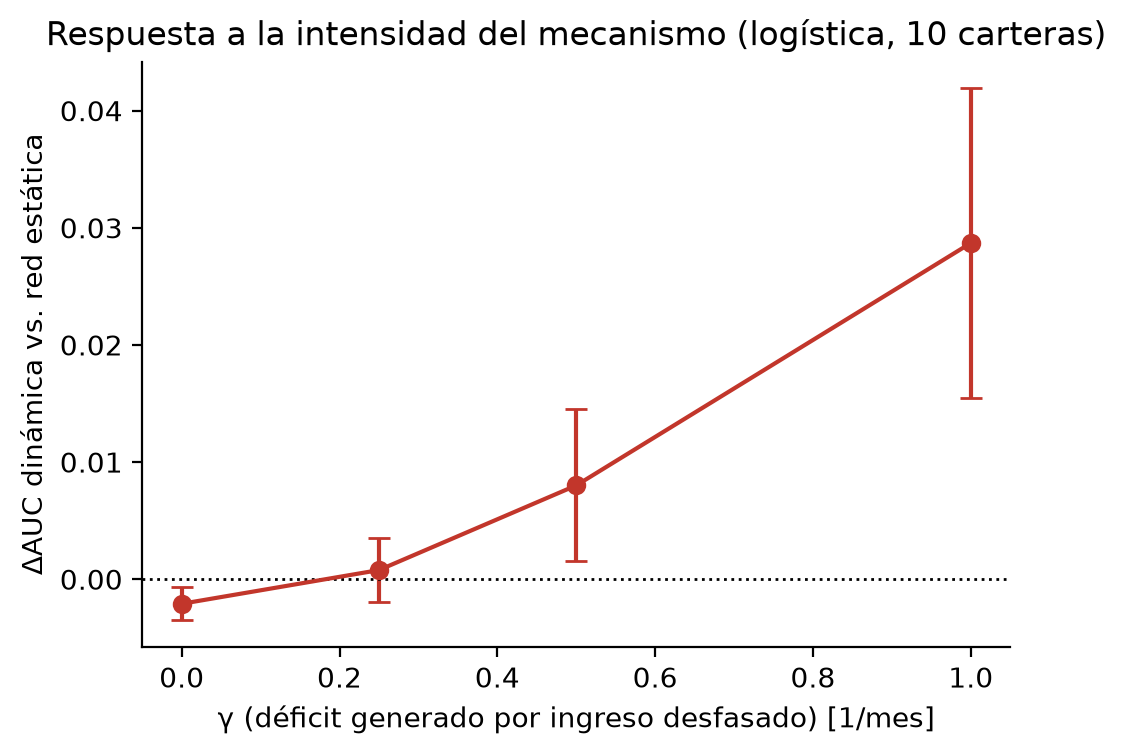
\includegraphics[width=\textwidth]{tarea6_sensibilidad_gamma.png}
\column{0.43\textwidth}
\centering
\begin{tabular}{cc}
\toprule
$\gamma$ & $\Delta$AUC \\
\midrule
0 & $-0.002$ \\
0.25 & $+0.001$ \\
0.5 & $+0.008$ \\
1.0 & $+0.029$ \\
\bottomrule
\end{tabular}
\vspace{0.3cm}

\small Con $\gamma=0$ el contagio sigue activo y aun así la dinámica no aporta.
\end{columns}
\clave{La señal viene de la desincronización, no del contagio.}
\end{frame}

\begin{frame}{El score clásico sigue siendo la base}
\begin{columns}[c]
\column{0.56\textwidth}
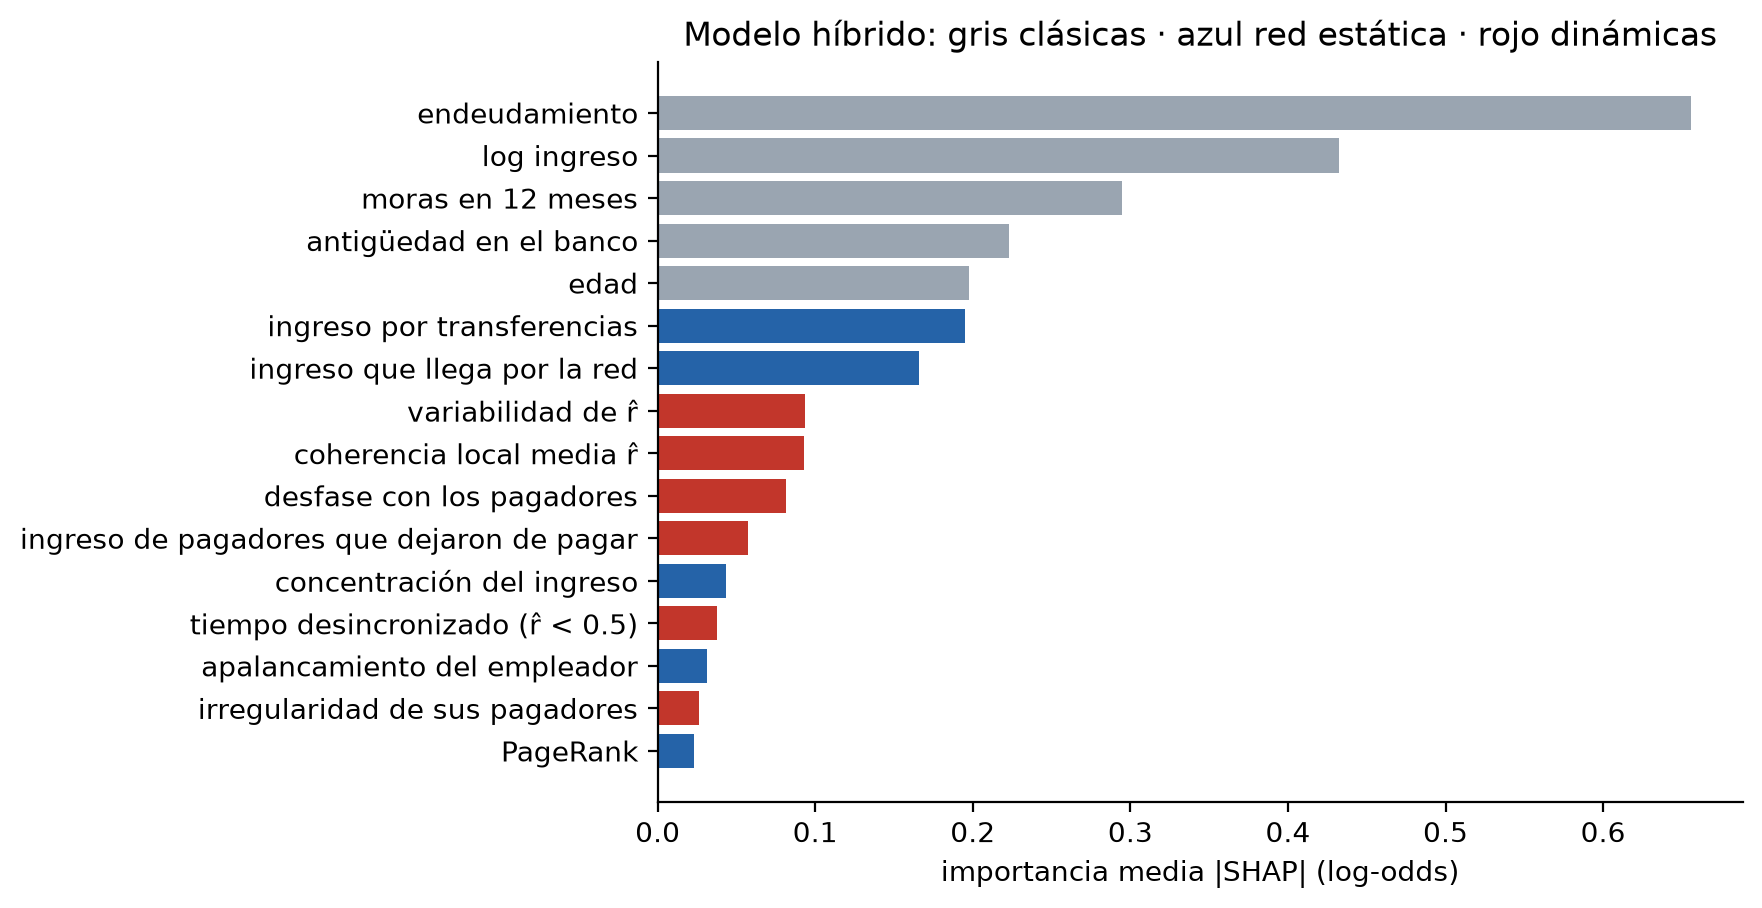
\includegraphics[width=\textwidth]{tarea6_shap.png}
\column{0.42\textwidth}
\small
\begin{itemize}
\item \textcolor{gris}{\textbf{Gris}}: clásicas. Pesan más (deuda, ingreso, mora).
\item \textcolor{azul}{\textbf{Azul}}: red estática.
\item \textcolor{rojo}{\textbf{Rojo}}: red dinámica. Destacan la variabilidad de $\hat r$,
su nivel y el desfase.
\end{itemize}
\end{columns}
\clave{El modelo híbrido complementa el score; no lo reemplaza.}
\end{frame}

\begin{frame}{Uso práctico: la quiebra de un empleador}
\begin{columns}[c]
\column{0.58\textwidth}
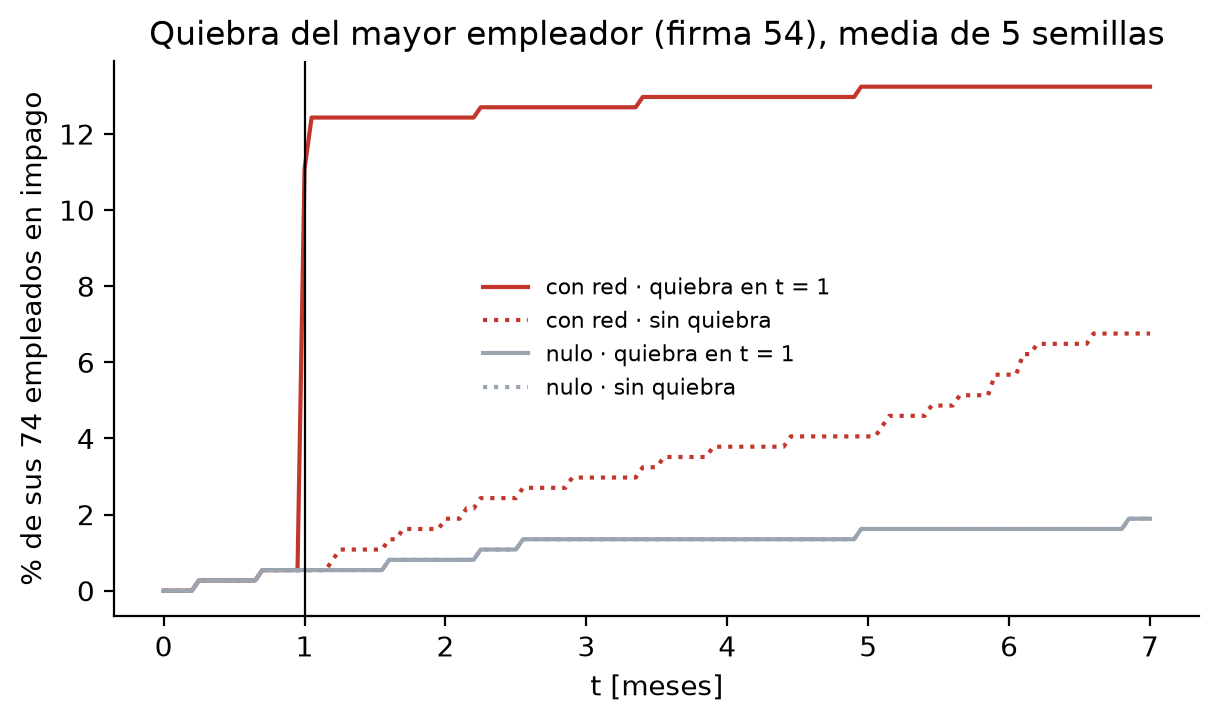
\includegraphics[width=\textwidth]{tarea6_quiebra.png}
\column{0.4\textwidth}
\small
\begin{itemize}
\item Quiebra la empresa con más empleados en el banco (74).
\item 12~\% de sus empleados cae de inmediato.
\item A 6 meses: 13~\% frente a 7~\% sin quiebra.
\item Mundo nulo: sin efecto.
\end{itemize}
\end{columns}
\clave{Sirve para pruebas de estrés por concentración en empleadores.}
\end{frame}

\begin{frame}{Qué demuestra y qué no}
\begin{columns}[T]
\column{0.48\textwidth}
\begin{exampleblock}{Demuestra}
\begin{itemize}
\item Si el mecanismo existe, se detecta con las transacciones del banco.
\item Aporta más que la red estática.
\item Desaparece sin mecanismo y crece con él.
\end{itemize}
\end{exampleblock}
\column{0.48\textwidth}
\begin{alertblock}{No demuestra}
\begin{itemize}
\item Que el mecanismo exista en un banco real.
\item El tamaño real del efecto (parámetros ilustrativos).
\item Qué pasa si el banco no ve toda la red.
\end{itemize}
\end{alertblock}
\end{columns}
\clave{El siguiente paso es una cartera real anonimizada.}
\end{frame}

% ===================================================================
\section{Cierre}

\begin{frame}{Software reproducible y aplicación web}
\begin{columns}[c]
\column{0.42\textwidth}
\small
\begin{itemize}
\item Python, 9 páginas en Streamlit.
\item Parámetros en archivos YAML, semillas fijas.
\item 127 pruebas automáticas.
\item Docker: corre igual en cualquier equipo.
\item Experimento completo: un comando, 20 s.
\end{itemize}
\column{0.56\textwidth}
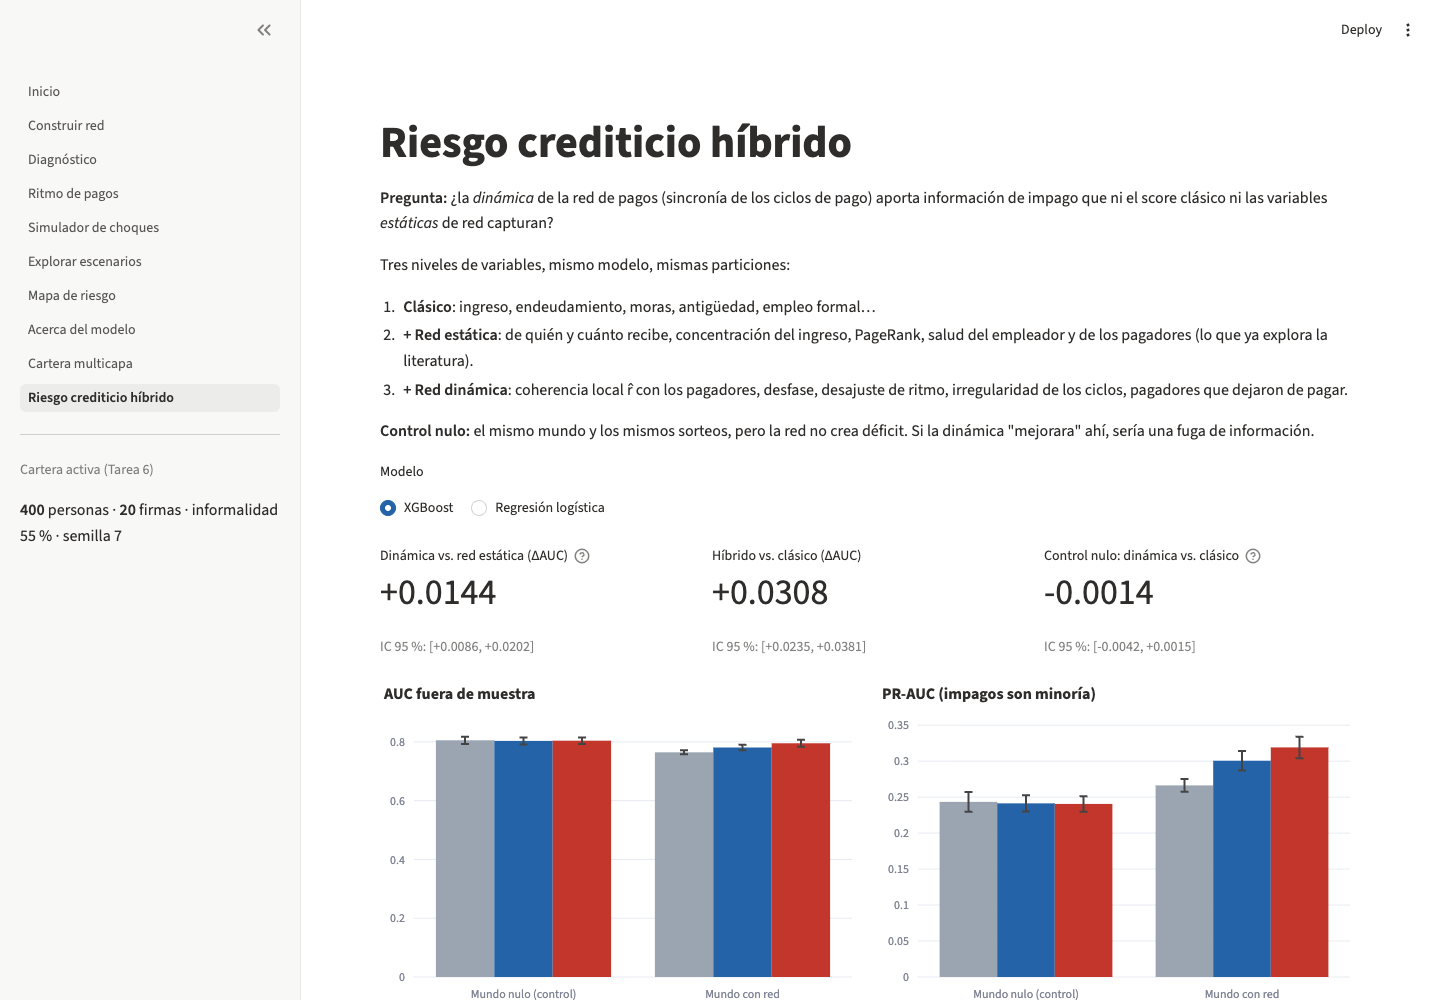
\includegraphics[width=\textwidth]{app_hibrido.png}
\end{columns}
\clave{Todo resultado de esta presentación se puede regenerar y explorar.}
\end{frame}

\begin{frame}{Conclusiones}
\begin{enumerate}
\item Un solo modelo une contagio, redistribución, sincronización y cascadas, y cada
parte se valida contra resultados exactos.
\item $R=\beta\rho(W)/\alpha$ indica si la red amortigua o amplifica.
\item El aprendizaje automático predice el colapso con AUC 0.98 en milisegundos.
\item \textbf{La sincronización de los pagos, medida con transacciones, mejora la
predicción del impago} más allá del score y de la red estática, y no lo hace en el
control nulo.
\end{enumerate}
\clave{No solo importa cuánto recibe un cliente, también cuándo.}
\end{frame}

\begin{frame}{Trabajo futuro}
\begin{enumerate}
\item \textbf{Datos reales}: aplicar el método a una cartera anonimizada.
\item \textbf{Fechas de cuota} como ritmo impuesto desde fuera.
\item \textbf{Retroalimentación}: el déficit también cambia el ritmo de pago.
\item \textbf{Visión parcial}: un banco frente al operador de Bre-B.
\end{enumerate}
\end{frame}

\begin{frame}[standout]
Gracias

\vspace{0.4cm}
\normalsize Preguntas
\end{frame}

% ===================================================================
\appendix
\section*{Respaldo}

\begin{frame}{Respaldo: modelo de la cartera multicapa}
\[
\dot x_i = -\alpha x_i + \sum_\ell\beta_\ell\sum_j\frac{W^\ell_{ij}}{s_i}x_j
+ \gamma\frac{k_i}{s_i}(1-r_i) + \sigma\xi_i(t)
\]
\[
\dot\theta_i = \omega_i + \sum_\ell K_\ell\sum_j\frac{W^\ell_{ij}}{k_i}\sin(\theta_j-\theta_i),
\qquad x_i^{(c)} = c\Bigl(\frac{\mathrm{PD}_\text{ref}}{\mathrm{PD}_i}\Bigr)^{\kappa}\varepsilon_i
\]
\footnotesize
\begin{tabular}{lll@{\hspace{1cm}}lll}
\toprule
Parámetro & Valor & Unidad & Parámetro & Valor & Unidad \\
\midrule
$\alpha$ & 1.0 & 1/mes & $\gamma$ & 0.5 & 1/mes \\
$\beta_{N,S,T}$ & 0.5, 0.4, 0.3 & 1/mes & $\lambda$ & 1.0 & meses de ingreso \\
$K_{N,S,T}$ & 0.8, 1.0, 0.3 & rad/mes & $\sigma$ & 0.3 & 1/$\sqrt{\text{mes}}$ \\
$c$, PD$_\text{ref}$, $\kappa$ & 1.1, 0.04, 0.35 & — & ventanas & 6 + 12 & meses \\
\bottomrule
\end{tabular}
\end{frame}

\begin{frame}{Respaldo: métricas completas (mundo con red)}
\footnotesize
\centering
\begin{tabular}{llcccccc}
\toprule
Mundo & Nivel & \multicolumn{2}{c}{AUC} & \multicolumn{2}{c}{PR-AUC} & KS & Brier \\
 & & log. & XGB & log. & XGB & log. & log. \\
\midrule
Con red & 1 · Clásico & 0.769 & 0.764 & 0.277 & 0.266 & 0.416 & 0.079 \\
Con red & 2 · + Estática & 0.784 & 0.781 & 0.307 & 0.301 & 0.437 & 0.077 \\
Con red & 3 · + Dinámica & 0.795 & 0.795 & 0.323 & 0.319 & 0.457 & 0.076 \\
\midrule
Nulo & 1 · Clásico & 0.810 & 0.805 & 0.255 & 0.243 & 0.487 & 0.050 \\
Nulo & 3 · + Dinámica & 0.809 & 0.804 & 0.252 & 0.241 & 0.486 & 0.050 \\
\bottomrule
\end{tabular}

\vspace{0.3cm}
\begin{tabular}{lcc}
\toprule
 & Nulo & Con red \\
\midrule
Clientes modelados & 40\,404 & 37\,431 \\
Impago a 12 meses & 5.9~\% & 9.6~\% \\
$R$ & 0 & 0.09–0.17 \\
\bottomrule
\end{tabular}
\end{frame}

\begin{frame}{Respaldo: calibración y relación sincronía--impago}
\begin{columns}[c]
\column{0.42\textwidth}
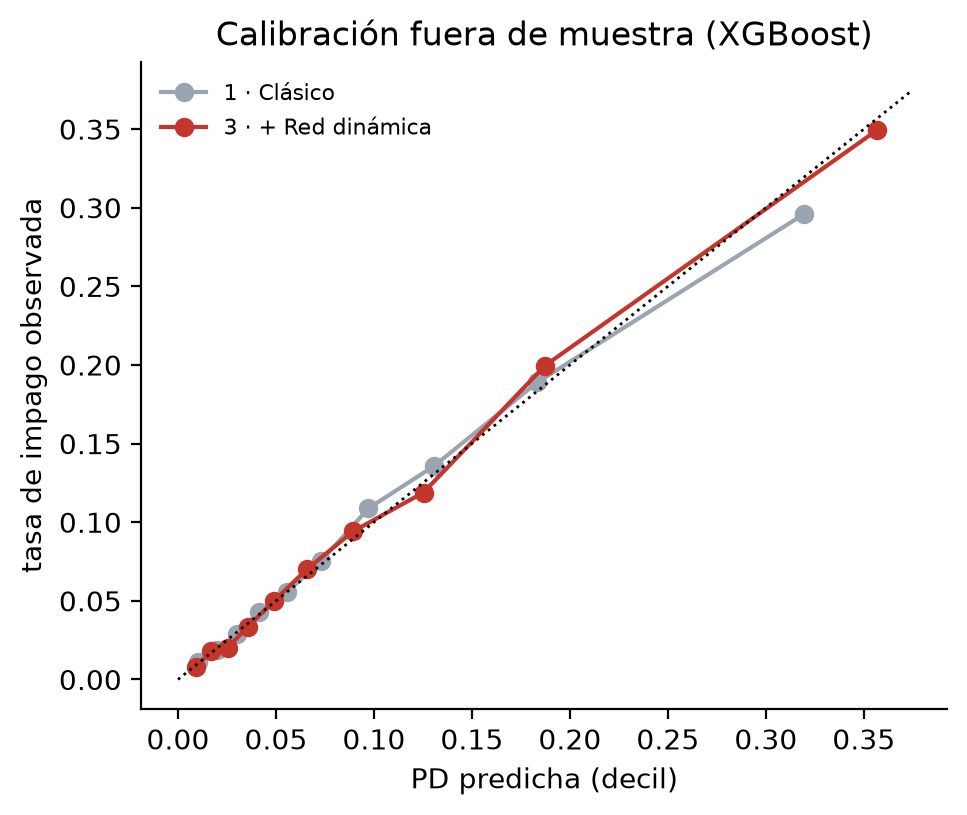
\includegraphics[width=\textwidth]{tarea6_calibracion.png}
\scriptsize Ambos modelos calibrados; decil de mayor riesgo: 35~\% (híbrido) frente a
30~\% (clásico) de impago observado.
\column{0.56\textwidth}
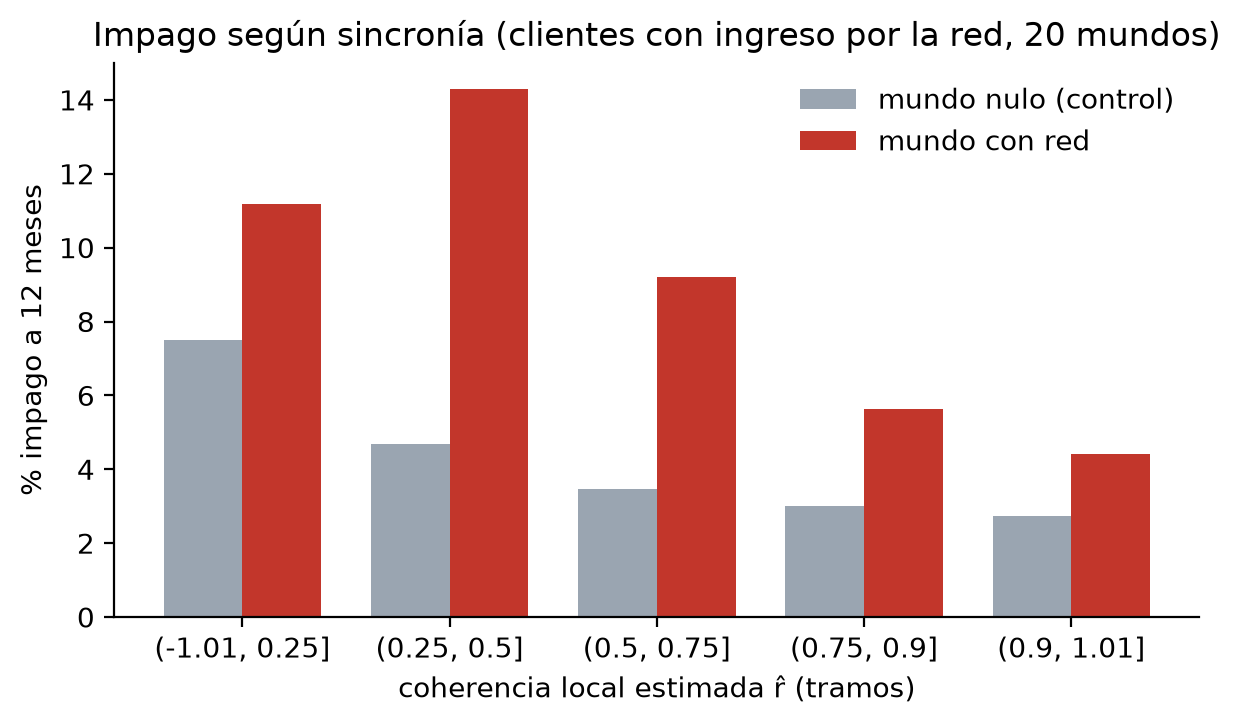
\includegraphics[width=\textwidth]{tarea6_impago_por_r.png}
\scriptsize Con red: 4.4~\% de impago con $\hat r>0.9$ y 11–14~\% con $\hat r<0.5$. En el
nulo el gradiente es menor y lo explica la informalidad.
\end{columns}
\end{frame}

\begin{frame}{Respaldo: redistribución y recuperación (tarea 2)}
\begin{columns}[c]
\column{0.4\textwidth}
\footnotesize
\begin{itemize}
\item $L=D_\text{out}-W$ conserva el déficit total (verificado a $10^{-10}$).
\item Estabilidad: $\sigma=\max\mathrm{Re}\,\lambda(M)$, con $M=-\alpha I-D_0L+\beta W$.
\item $\tau_\text{rec}=-1/\sigma$; en redes simétricas, tasa $\alpha+D_0\lambda_2$ (1~\%).
\end{itemize}
\column{0.58\textwidth}
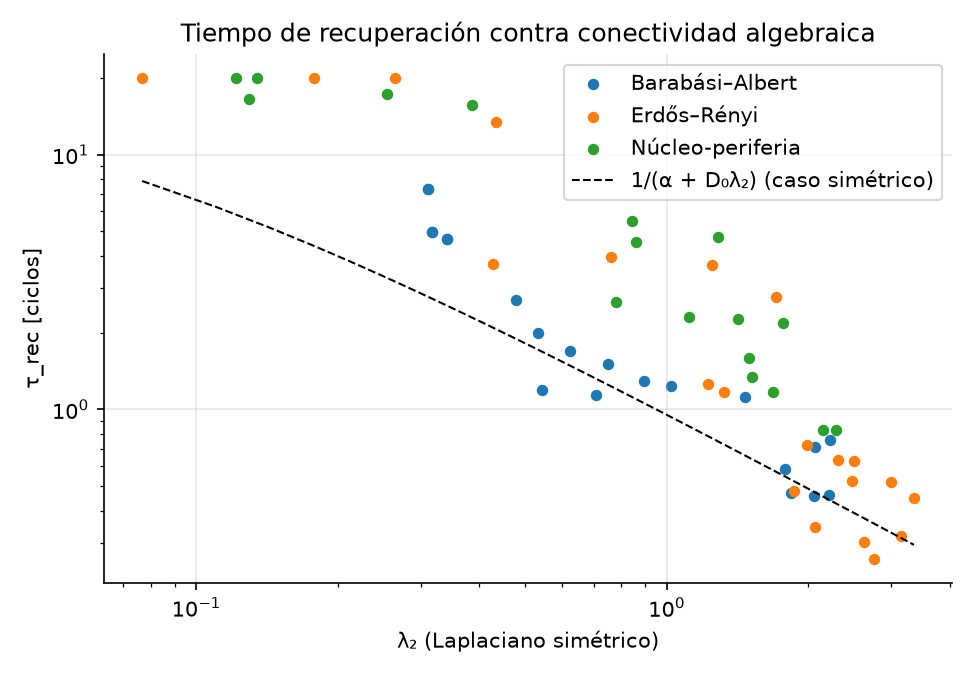
\includegraphics[width=0.49\textwidth]{fase2_tau_vs_lambda2.png}\hfill
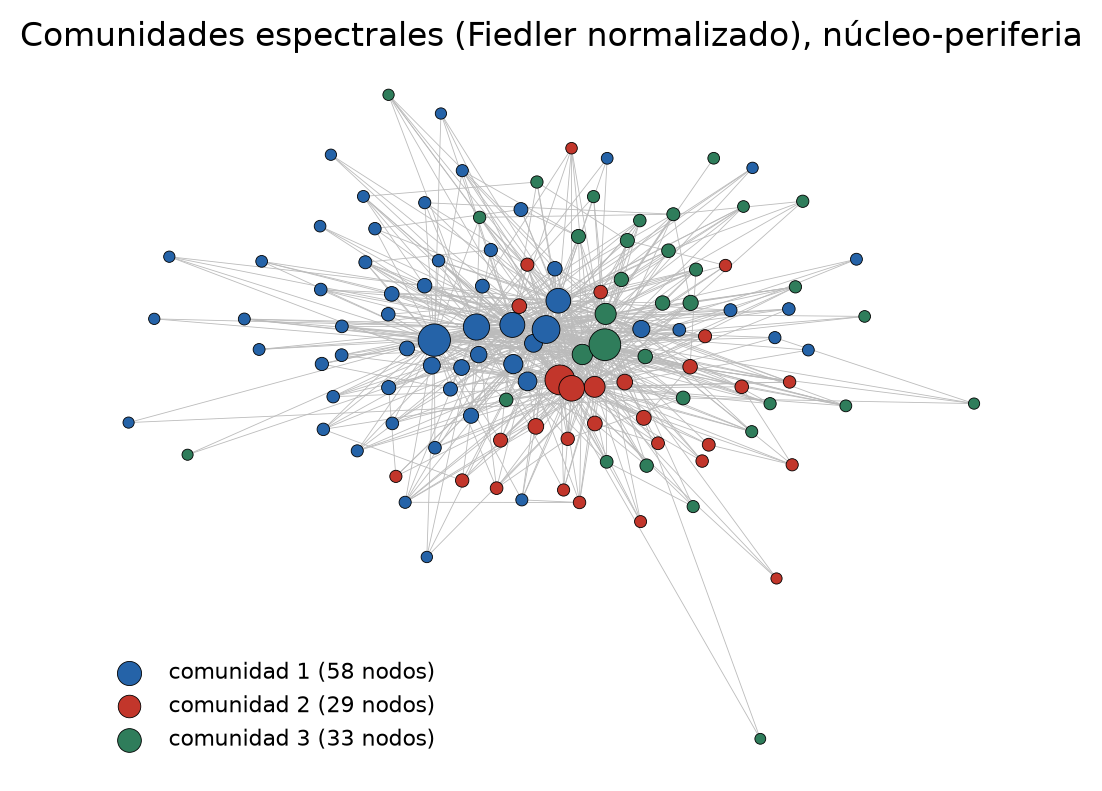
\includegraphics[width=0.49\textwidth]{fase2_comunidades_normalizado.png}
\end{columns}
\end{frame}

\begin{frame}{Respaldo: tarea 5 en detalle}
\begin{columns}[c]
\column{0.5\textwidth}
\footnotesize
\begin{tabular}{lll}
\toprule
Modelo & Objetivo & Desempeño \\
\midrule
Logística & colapso & AUC 0.957 · PR 0.741 \\
XGBoost & colapso & AUC 0.980 · PR 0.880 \\
XGBoost & cascada & $R^2$ 0.50 · $\rho_s$ 0.30 \\
GCN & cascada & $R^2$ 0.60 · $\rho_s$ 0.29 \\
\bottomrule
\end{tabular}

\vspace{0.3cm}
\small Hipercubo latino de 13 parámetros, más densidad cerca de $R=1$, GroupKFold por red.
\column{0.48\textwidth}
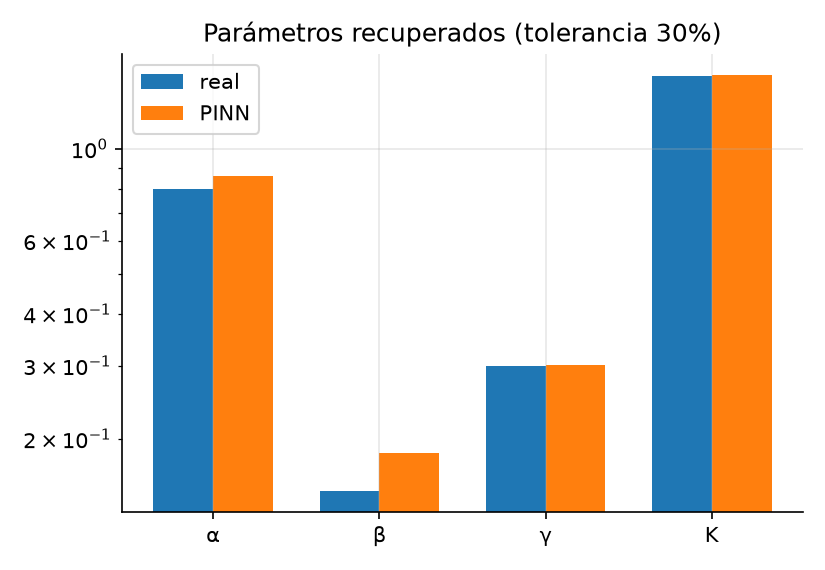
\includegraphics[width=\textwidth]{fase6_pinn_parametros.png}
\scriptsize PINN: error $<1~\%$ en $\gamma$ y $K$; 7~\% en $\alpha$; 23~\% en $\beta$.
\end{columns}
\end{frame}

\begin{frame}{Respaldo: referencias principales}
\scriptsize
\begin{columns}[T]
\column{0.5\textwidth}
\begin{itemize}
\item Acebrón et al. (2005). The Kuramoto model. \emph{Rev.\ Mod.\ Phys.}
\item Battiston et al. (2012). DebtRank. \emph{Sci.\ Rep.}
\item Boccaletti et al. (2014). Multilayer networks. \emph{Phys.\ Rep.}
\item Eisenberg y Noe (2001). \emph{Management Science}.
\item Kipf y Welling (2017). GCN. \emph{ICLR}.
\item Letizia y Lillo (2019). \emph{EPJ Data Science}.
\item Lundberg y Lee (2017). SHAP. \emph{NeurIPS}.
\end{itemize}
\column{0.5\textwidth}
\begin{itemize}
\item Newman (2010). \emph{Networks}. Oxford.
\item Óskarsdóttir y Bravo (2021). \emph{Omega}.
\item Pikovsky, Rosenblum y Kurths (2001). \emph{Synchronization}.
\item Raissi, Perdikaris y Karniadakis (2019). PINN. \emph{J.\ Comput.\ Phys.}
\item Rodrigues et al. (2016). \emph{Phys.\ Rep.}
\item Shi y Malik (2000). \emph{IEEE TPAMI}.
\item Watts (2002). \emph{PNAS}.
\end{itemize}
\end{columns}
\end{frame}

\end{document}
